\documentclass[11pt,oneside]{article}
\usepackage{amsmath}
\usepackage{pdfpages}
\usepackage{appendix}
\usepackage{natbib}
% \usepackage{amssymb}
\usepackage{makeidx}
\usepackage{graphicx}
\usepackage{epstopdf}
\usepackage{float}
\usepackage{mdwlist}
\usepackage{bm}
\usepackage{fullpage}

\begin{document}
\title{Exploring non-linear inversions: a 1D magnetotelluric example}
\author{Seogi Kang, Lindsey J. Heagy, Rowan Cockett, and Douglas W. Oldenburg}

\maketitle
At some point in many geophysical workflows, an inversion is a necessary step for answering the geoscientific question at hand: whether it is recovering a reflectivity series from a seismic trace in a deconvolution problem, finding a susceptibility model from magnetic data, or recovering conductivity from an electromagnetic survey. This is particularly true when working with data sets where it may not even be clear how to plot the data: 3D direct current resistivity and induced polarization surveys (it is not necessarily clear how to organize data into a pseudosection) or multi-component data, such as electromagnetic data (we can measure three spatial components of electric and/or magnetic fields through time over a range of frequencies). Inversion is a tool for translating these data into a model we can interpret. The goal of the inversion is to find a ``model'', some description of the earth’s physical properties, that is consistent with both the data and geologic knowledge.

In a general inverse problem, we start from a forward problem, of the form $\mathcal{F}[\mathbf{m}] = \mathbf{d}$, where $\mathcal{F}$ is the forward operator (the mathematical description of the physics/problem), $\mathbf{d}$ is our data, and $\mathbf{m}$ is our earth model (an array of numbers that describes the physical properties of the earth). Matt Hall kicked off the discussion of inversions in the Leading Edge in his \emph{Linear Inversion} tutorial \citep{HallTutorial}. He walked through how to solve the classic linear inverse problem, where the forward simulation takes the form $\mathcal{F}[\mathbf{m}] = \mathbf{G}\mathbf{m} = \mathbf{d}$. The example he demonstrated is a deconvolution problem, in that case, $\mathbf{G}$ is a convolution matrix, $\mathbf{m}$ is the reflectivity series and $\mathbf{d}$ is a seismic trace. He introduced the concepts of an underdetermined problem, motivated the need for regularization, formulated the inversion in terms of an optimization problem and solved the linear inverse problem (in true polyglot fashion, using Python, Lua, Julia, and R!). In this tutorial, we will pick up from there and explore a \emph{nonlinear} forward problem, of the form $\mathcal{F}[\mathbf{m}] = \mathbf{d}$; in this case, our forward operator is a function of the model. In the attached notebooks, we use SimPEG (http://simpeg.xyz) for the implementation in Python of the physics simulations, optimization, and structure necessary to perform an inversion \citep{SimPEGPaper}.

\section{Magnetotellurics}
We will explore the 1D magnetotelluric (MT) survey technique, which is a natural source electromagnetic method. In magnetotellurics, plane-wave source-fields are generated by solar wind (giving us low frequency signals $<$ 1 Hz) and lightning strikes worldwide (giving us higher frequency signals $>$ 1 Hz). In magnetotellurics, the model $\mathbf{m}$ is a description of the earth’s electrical conductivity $\sigma$ and $\mathcal{F}[\mathbf{m}]$ solves Maxwell’s equations --- giving the electric field $\vec{E}$ and the magnetic field $\vec{H}$ --- for a plane wave source. In the continuous world, Maxwell’s equations are:
\begin{equation}
\begin{split}
\nabla \times \vec{E} + i\omega\mu\vec{H} &= 0 \\
\nabla \times \vec{H} - \sigma\vec{E} &= 0 \\
\text{with boundary conditions}
\end{split}
\label{eq:maxwell}
\end{equation}
where $\mu$ is magnetic permeability, generally taken to be the permeability of free space $\mu_0$, and $\omega = 2 \pi f$ is the angular frequency ($f$ is frequency in Hz). When we discretize Maxwell's equations so that they can be solved numerically (see the first notebook), we obtain a matrix system of the form
\begin{equation}
    \mathbf{A}(\mathbf{m})\mathbf{u} = \mathbf{b}
    \label{eq:discreteMaxwell}
\end{equation}
where $\mathbf{A}(\mathbf{m})$ is a matrix capturing the physics, $\mathbf{u}$ is vector of the electric and magnetic fields everywhere in our simulation domain, and $\mathbf{b}$ includes the boundary conditions that describe the plane wave source. This problem is nonlinear because this matrix $\mathbf{A}$ depends on the conductivity model. When we solve equation \ref{eq:discreteMaxwell} for $\mathbf{u}$, we obtain the electric and magnetic fields everywhere on our mesh. Our data consist of samples of the electric and magnetic fields where we have receivers. For the MT problem, the measured data, $\mathbf{d}$, are impedances; for the 1D problem, the impedance $Z_{xy}$ at a single frequency is given by
\begin{equation}
Z_{xy} = -\frac{E_x}{H_y}.
\label{eq:impedance}
\end{equation}
Note that the impedance is a complex number, consisting of real and imaginary parts. Impedance is a non-intuitive quantity; often, we instead consider apparent resistivity\footnote{Note that resistivity is the inverse of conductivity $\rho = 1/\sigma$} $\rho_\mathrm{a}$ and phase $\psi$, given by
\begin{equation}
\rho_\mathrm{a} = \frac{1}{\mu_0\omega} \big|Z_{xy}\big|^2,
\quad
\psi = \tan^{-1}\left(\frac{\text{Im}(Z_{xy})}{\text{Re}(Z_{xy})}\right).
\label{eq:rhoa_phase}
\end{equation}
For an earth that is a half-space, the apparent resistivity equals the true resistivity, and the phase is $45^{\circ}$. When we implement the computation of the data, we define a method that (a) selects the values of the electric and magnetic fields at the surface of the earth from the fields that we computed everywhere in our domain $\mathbf{u}$, and (b) computes their ratio to provide us with impedance data, that is:  $\mathbf{P}(\mathbf{u}) = \mathbf{d}$.


In summary, to implement the forward simulation for the MT problem ($\mathcal{F}[\mathbf{m}] = \mathbf{d}$), we break it into two steps:
\begin{enumerate}
     \item Solve $\mathbf{A}(\mathbf{m})\mathbf{u} = \mathbf{b}$
    \item Compute the impedance data $\mathbf{d} = \mathbf{P}(\mathbf{u})$
\end{enumerate}
In the first notebook, we provide details on how each step is performed using a finite difference approach, and if you are looking for more on numerical discretization, we wrote a tutorial on finite volume methods \citep{Cockett2016}.

The inversion aims to solve $\mathcal{F}^{-1}[\mathbf{d}]$ for a model. Just as in the linear problem, we require regularization in order to select a model from the infinitely many that can fit the data. Before we tackle this \emph{ill posed} inverse problem, let's explore an example of nonuniqueness: how can different models give us the same data?

\section{Go forwards}

A classic example that demonstrates the non-uniqueness of MT data is the equivalence of the conductivity-thickness product (conductance) of a thin layer. If we start with a layer that has a conductivity of $\sigma$, halve its thickness and double its conductivity, the resulting data will be similar. In Figure \ref{fig:sigmat}, we show apparent resistivity and phase data for five models, each of which has the same conductance. In all of the simulations, the data shows a decrease in apparent resistivity and an increase in phase starting at $\sim$10Hz. Thus, in all of the data we have evidence of a conductive layer, and the frequency range at which it appears is an indicator of the depth of the layer (you can explore by changing the \texttt{depth} variable in the model setup of the second notebook). However, all scenarios produce similar data. Even with a small amount of noise, we cannot expect an inversion code to separate the conductivity and thickness of a conductive unit without incorporating additional information. When setting up the inverse problem and defining regularization (next up!), it is important to realize that the choices we make there will influence the character of the model we recover, as the data alone do not provide us with a unique model.

\begin{figure}[htb!]
    \centering
    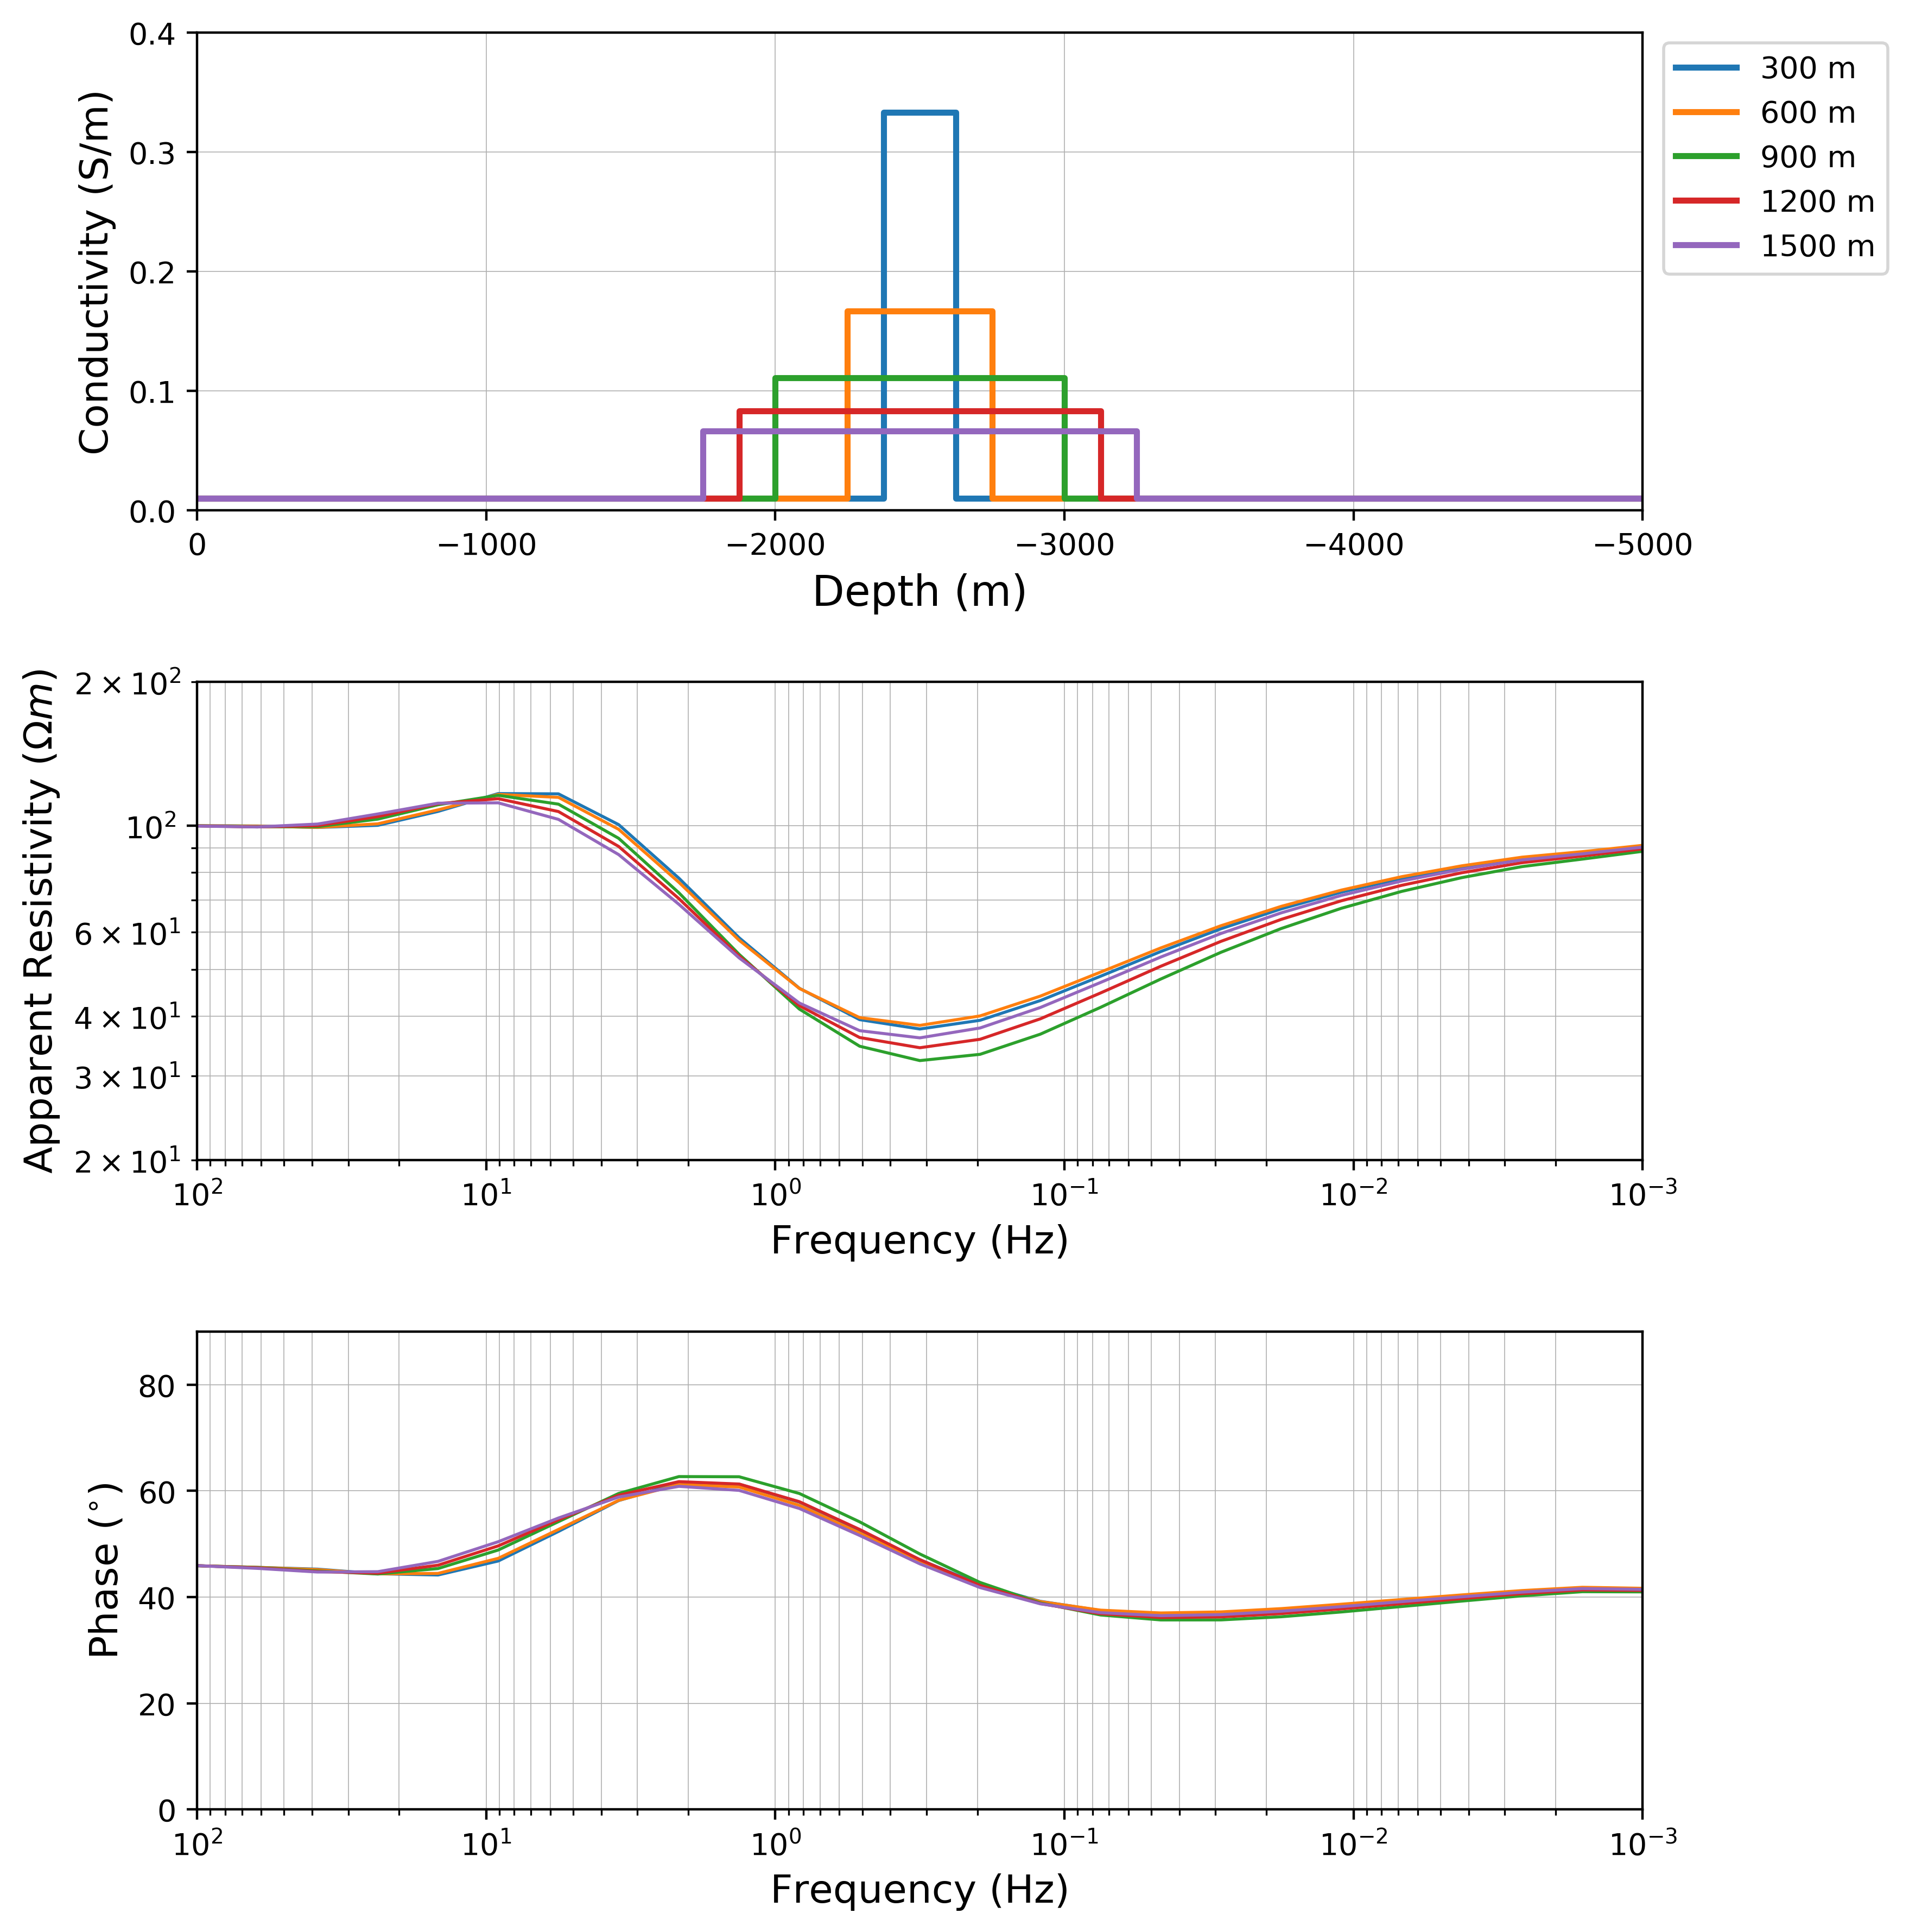
\includegraphics[width=\textwidth]{images/sigmat.png}
\caption{Magnetotelluric responses from five models, each having an equivalent conductivity-thickness product for the conductive layer. (a) Conductivity models, (b) apparent resistivity ($\rho_a$), and (c) phase ($\phi$).}
\label{fig:sigmat}
\end{figure}

\section{Go backwards}

There are many models that can fit the data, so we need a means of \emph{regularizing} our inversion so that we can select a single, reasonable model from the (infinitely!) many that agree with the data. We will come back to how the regularization $\phi_{\text{m}}$ is defined, but for now, consider it as a measure of how ``reasonable'' the model is based upon our prior knowledge about the earth. Formally, we pose the inversion as an optimization problem:
\begin{equation}
\begin{split}
\underset{\mathbf{m}}{\text{minimize}} \quad &\phi_\text{m}(\mathbf{m}) \\
\text{subject to }\quad &\mathcal{F}[\mathbf{m}] = \mathbf{d}_{\text{obs}}
\end{split}
\end{equation}
Essentially we are saying ``find the model $\mathbf{m}$ that best fits the assumptions we are making in the regularization $\phi_\text{m}(\mathbf{m})$, and that agrees with the observed data $\mathbf{d}_{\text{obs}}$.'' In practice, our data are noisy, so there is no sense in fitting them exactly. Rather, we pose the optimization problem as a trade-off between fitting the data and fitting the regularization, so our inverse problem can be stated as:

\begin{equation}
\underset{\mathbf{m}}{\text{minimize}} \quad \phi(\mathbf{m}) = \phi_\mathrm{d}(\mathbf{m}) + \beta\phi_\mathrm{m}(\mathbf{m})
\end{equation}
where $\phi_d(\mathbf{m})$ is the data misfit, a measure of how far our simulated data are from the observed data; $\phi_m(\mathbf{m})$ is the regularization; and $\beta$ is a trade-off parameter that weights the relative importance of the data misfit and regularization in the optimization. A larger $\beta$ says that we want our model to do a good job minimizing the regularization, while a smaller $\beta$ turns down the volume of the regularization and says that fitting the data is more important in the inversion.

The data misfit is often taken to be a weighted $\ell_2$ norm:
\begin{equation}
\phi_d(\mathbf{m}) = \frac{1}{2}\|\mathbf{W_d} (\mathcal{F}(\mathbf{m}) - \mathbf{d}_{\text{obs}})\|^2_2
\end{equation}
where $\mathbf{W_d}$ captures the noise model (typically it is a diagonal matrix containing the standard deviation of each datum).

The regularization is one place where \emph{a priori} information about the geologic setting can be brought in. There are a variety of regularization functionals that can be chosen, but one of the most widely used is Tikhonov regularization, which again uses $\ell_2$ norms:
\begin{equation}
\phi_m(\mathbf{m}) = \frac{1}{2}\big(\alpha_\mathrm{s}\|\mathbf{W_\mathrm{s}} (\mathbf{m} - \mathbf{m}_{\text{ref}})\|^2_2 + \alpha_\mathrm{z}\|\mathbf{W_\mathrm{z}} (\mathbf{m})\|^2_2 \big)
\end{equation}
The first term is often referred to as the "smallness" as it measures the "size" of the model (in the $\ell_2$ sense). The matrix $\mathbf{W_\mathrm{s}}$ is generally taken to be a diagonal matrix that may contain information about the length scales of the model or be used to weight the relative importance of various parameters in the model. The scalar $\alpha_s$ weights the relative importance of this term in the regularization. Notice that we include a reference model, $\mathbf{m}_{\text{ref}}$. Often this is defined as a constant value, but if more information is known about the background, that can be used to construct a more intricate reference model. Here, we will not delve too far into how the reference model impacts the recovered results, but you are encouraged to change \texttt{mref} in the notebooks and investigate its impact.

The second term is often referred to as the "smoothness". The matrix $\mathbf{W_\mathrm{z}}$ approximates the derivative of the model with respect to depth, and is hence a measure of how "smooth" the model is. The term $\alpha_\mathrm{z}$ weights the relative importance of smoothness in the regularization.

From this setup, we see that there are quite a number of choices to make: defining uncertainties on the data ($\mathbf{W_\mathrm{d}}$), selecting a reference model ($\mathbf{m}_{\text{ref}}$), choosing the importance of smallness and smoothness ($\alpha_\mathrm{s}$ and $\alpha_\mathrm{z}$), and selecting a trade-off parameter ($\beta$). Let’s start by assuming a known noise model, fix $\alpha_\mathrm{s}$ and $\alpha_\mathrm{z}$, and explore the impact of the trade-off parameter $\beta$. Our forward problem depends upon the electrical conductivity. For the inverse problem, however, we are free to use any function of the conductivity as a parameter. The electrical conductivity of earth materials varies by many orders of magnitude and is strictly positive. Thus it is advantageous to use $\mathbf{\log(\sigma)}$ as the model in the inverse problem. For a nonlinear problem, we also have the additional choice of the initial model $\mathbf{m}_0$ at which to start the inversion. Although we will not discuss the choice of $\mathbf{m}_0$, you are encouraged to change the initial model in the notebooks and examine the impact it makes because it can be significant!

\subsection{The $\beta$ knob}
If the noise is Gaussian, then the sum of squares (our data misfit) is a Chi-squared distribution, which has an expected value of $N_\text{data}$ (in our case, we divide this by two to match our definition of $\phi_\mathrm{d}$). Thus, the ideal choice of $\beta$ is one that gives us $\phi_\mathrm{d}^* \approx \frac{1}{2} N_\text{data}$. To demonstrate the effect of $\beta$, we consider a five layer model, originally shown in \cite{Monographs}, and will demonstrate inversions when we achieve the target misfit, underfit the data and overfit fit the data. The conductivity model used is the solid black line in Figure \ref{fig:beta_knob}a. For these inversions we fix the regularization parameters to $\alpha_\mathrm{s} = 10^{-2}$, $\alpha_\mathrm{z} = 1$ and set $\mathbf{m}_{\text{ref}} = 10^{-2} S/m$, and the initial model, $\mathbf{m}_0 = \mathbf{m}_{\text{ref}}$ (feel free to change them in the notebook!). We start the inversion with a large $\beta$ and decrease its value to plot the trade-off or Tikhonov curve (Figure \ref{fig:beta_knob}b). In blue, we show the inversion that is stopped when the data misfit approximately equals the  target misfit (the star in Figure \ref{fig:beta_knob}b). Figures \ref{fig:beta_knob}c and \ref{fig:beta_knob}d show the data as apparent resistivity and phase, which is a visualization of our complex-valued impedance data. The blue line in Figure \ref{fig:beta_knob}a shows the recovered model, which identifies the general structure and conductivity values of the five layers. In this case, we are employing a smooth regularization, thus we expect to recover smoothly varying structures.


\begin{figure}[htb!]
    \centering
    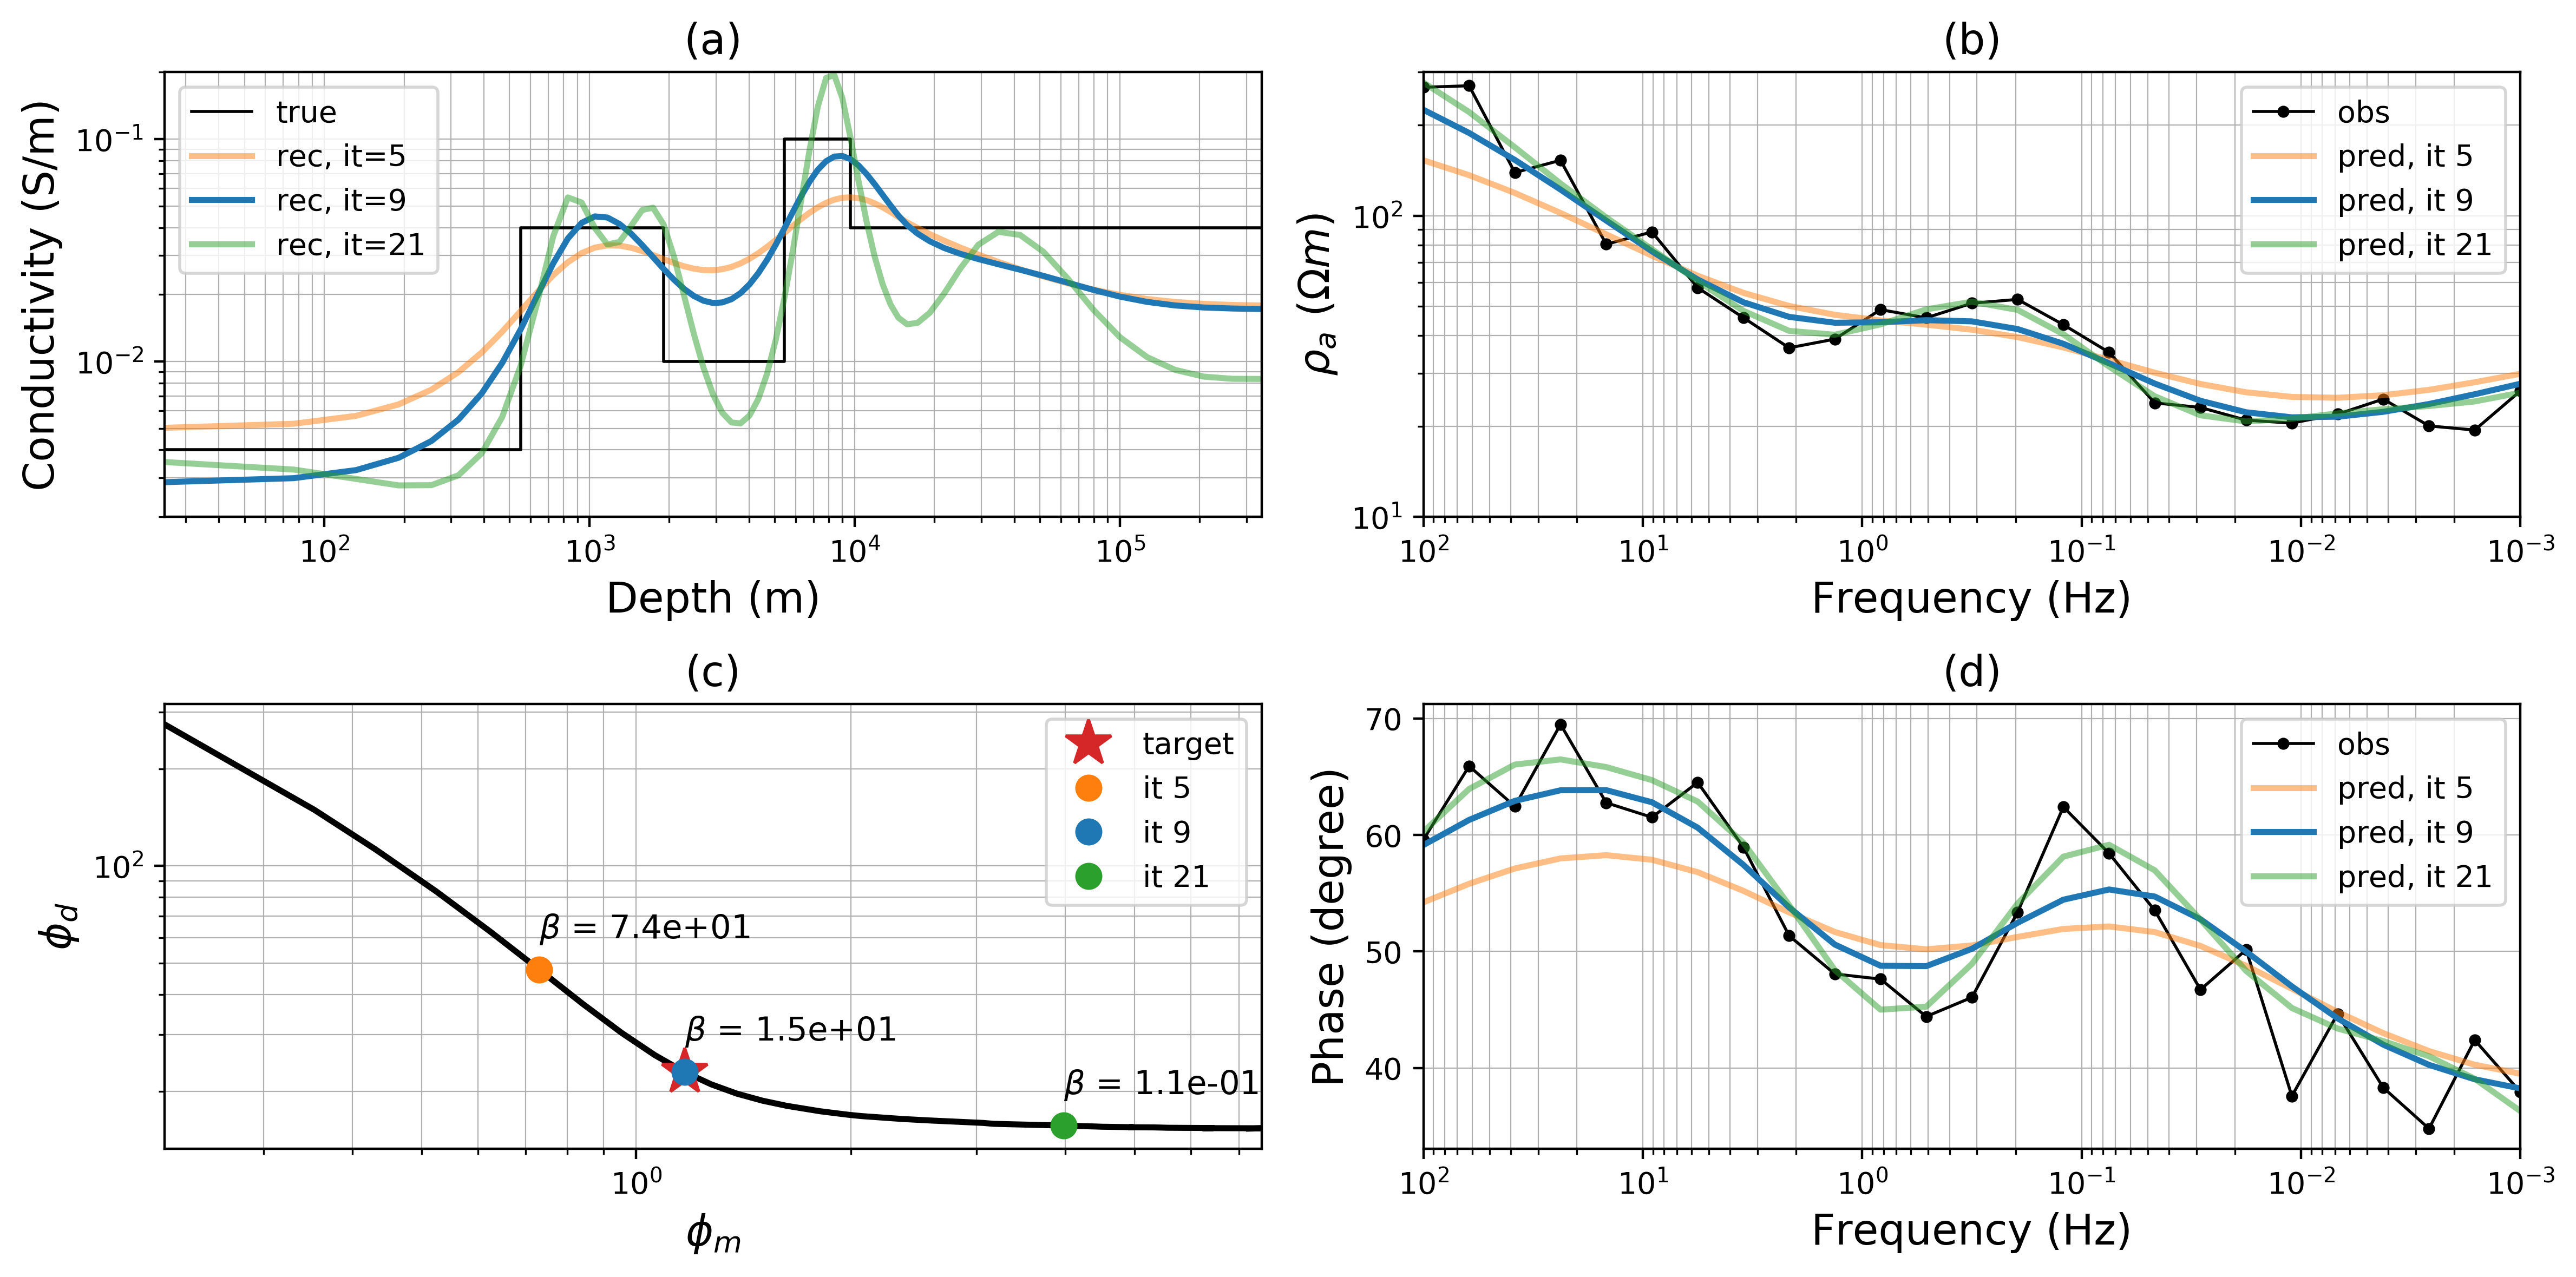
\includegraphics[width=\textwidth]{images/beta_knob.png}
\caption{Inversions which fit the data (blue), underfit the data (orange), and overfit the data (green). (a) True (black) and recovered electrical conductivity models. (b) Tikhonov curve showing the trade off between the misfit and regularization, target misfit (red star), and achieved misfit corresponding to each of the inversion results shown (c) observed (black) and predicted apparent resistivity data, (d) observed (black) and predicted phase data.}
\label{fig:beta_knob}
\end{figure}

If we instead choose a larger $\beta$, reducing the contribution of the data misfit to the objective function, we underfit the data, as is shown in orange in Figure \ref{fig:beta_knob}. Although we still see evidence of two conductive structures, we do not recover their amplitudes, and do a poor job resolving the location and widths of the conductive layers (if you had to pick the top of the first layer, where should it be?). Examining the plots in \ref{fig:beta_knob}c and d, there is more insight about the subsurface conductivity that can be learned by pushing the inversion to extract more from the data.

On the other extreme, we can choose a very small $\beta$, and try to fit all of the details in the data. Doing this, we obtain the results shown in green in Figure \ref{fig:beta_knob}. When we push the inversion to fit the (noisy!) data very closely, we end up fitting the noise. In order to do this, conductivity contrasts are exaggerated and oscillatory and erroneous conductivity structures are introduced in the inversion.


\subsection{The $\alpha$ knobs}

For the inversions shown in Figure \ref{fig:beta_knob}, we prescribed the values the $\alpha_s$, $\alpha_z$. What impact do they have on the character of the model we recover?

In Figure \ref{fig:alphas}, we compare two inversions with different regularization parameters: (1) a ``smooth'' inversion (blue line), with $\alpha_s = 10^{-5}$ and $\alpha_z = 1$, and (2) a ``small'' inversion (orange line): with $\alpha_s = 1$ and $\alpha_z = 10^{-5}$. In both, $\beta$ was chosen so that a desired target misfit was achieved. The smooth inversion penalizes large gradients; the resulting model has two smooth peaks. Note that we smooth over the resistive third layer, over-estimating its conductivity. The ``small'' inversion instead favors models that are close to the reference model; this model has more structure. The resistivity of the first layer matches well (the conductivity of the first layer is equivalent to our reference model) and the conductivity of the third layer is closer to its true value, but additional oscillatory structures are introduced at depth. In the third notebook, you can explore the impact of these parameters yourself!

\begin{figure}[htb!]
    \centering
    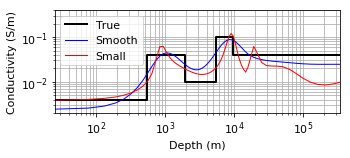
\includegraphics[width=\textwidth]{images/alphas.png}
\caption{Comparing the use of Smooth regularization versus Small regularization in the inversion.}
\label{fig:alphas}
\end{figure}


In practice, these parameters are often determined by experimentation; strategies such as examining length scales are often successfully adopted (see page 38 in  \cite{OldenburgTutorial}). Changing the relative values of $\alpha_s$ and $\alpha_z$ is one way to bring in a priori information. If we know very little, often starting with a smooth inversion is a good option; this penalizes structure (high gradients) while showing general trends. If more structure is expected, or a reliable reference model can be built from additional data such as physical property measurements, well logs, or additional geophysical/geologic data, then the influence of the smallness term may be increased. There are a few other ways to bring in additional a-priori information. If we are expecting a more ``blocky'' model, we can choose a different norm (such as an $\ell_1$ norm), or if we have structural constraints, we can introduce other weighting structures (e.g. on the smoothness); these are knobs for another tutorial and there is discussion in \cite{OldenburgTutorial}.
\section{Summary}
In this tutorial, we have introduced the forward simulation for magnetotellurics and explored a few aspects of the inverse problem. Prior to jumping into an inversion, it is important to know the limitations of the survey and data, and what you can and cannot resolve, even if there is no noise! Forward modelling is a powerful tool for setting realistic expectations of an inversion.

To set up and solve the inverse problem,  we posed the inversion as an optimization problem that searches for a model of the earth that minimizes an objective function consisting of a data misfit and a regularization term. There are many choices to be made in defining the various elements of the inverse problem, including how to assign uncertainties, selecting a trade-off parameter, defining the regularization function, and choosing initial and reference models. In this tutorial we explored two of the knobs: (1) the trade-off parameter and (2) the relative importance of smallness and smoothness contributions in Tikhonov regularization. The interactive notebooks that are provided allow you to change parameters and experiment with their impact.



\clearpage
\bibliographystyle{seg}  % style file is seg.bst
\bibliography{references.bib}

\end{document}
